
\begin{frame}
    \frametitle{Ring configurations}
    \begin{definition}
        A planar graph $\confg = R_n + \core$ consisting of a ring $R_n$ and an interior $\core$ is called a \emph{ring configuration} on $R_n$. $\core$ is called the \emph{core} of $\confg$.
    \end{definition}

    \begin{figure}[!h]
        \centering
            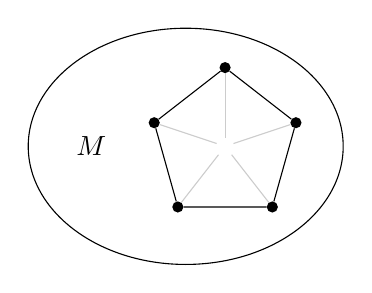
\begin{tikzpicture}
            \draw[fill=white] (-0.5, 0) ellipse (2cm and 1.5cm);
            %\draw[fill=lightgray, draw=black] (0,0) circle (1.25cm);
            %\draw[fill=white] (0,0) circle (0.75cm);
            \node at (-0.7, 0.9) {$\confg$};
            \node at (-1.7, 0) {$M$};
    
            \node[inner sep=1mm] (c) at (0, 0) {$\core$};
            \node[circle, fill, scale=0.015cm] (l1) at (0, 1) { };
            \node[circle, fill, scale=0.015cm] (l2) at (0.9, 0.30) { };
            \node[circle, fill, scale=0.015cm] (l3) at (0.6, -0.77) {};
            \node[circle, fill, scale=0.015cm] (l4) at (-0.6, -0.77) {};
            \node[circle, fill, scale=0.015cm] (l5) at (-0.9, 0.30) {};
    
            \draw[opacity=0.2] (c) -- (l1);
            \draw[opacity=0.2] (c) -- (l2);
            \draw[opacity=0.2] (c) -- (l3);
            \draw[opacity=0.2] (c) -- (l4);
            \draw[opacity=0.2] (c) -- (l5);
            \draw (l1) -- (l2) -- (l3) -- (l4) -- (l5) -- (l1);
        \end{tikzpicture}
    \end{figure}

    We have already shown reducibility if $\core = \varnothing$ (nothing)!
\end{frame}

\begin{frame}
    \frametitle{Finding common ring colorings}

    We split our graph into $M+R$ and $\core+R$. Now we try to find a common coloring on the ring $R$.
    \begin{figure}[!h]
        \centering
        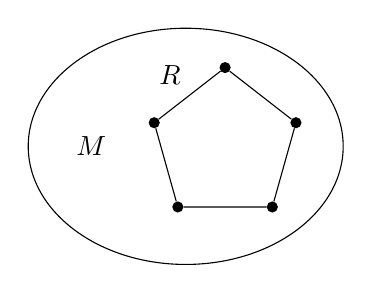
\begin{tikzpicture}
            \draw[fill=white] (-0.5, 0) ellipse (2cm and 1.5cm);
            \node at (-1.7, 0) {$M$};
            \node at (-0.7, 0.9) {$R$};
    
            \node[circle, fill, scale=0.015cm] (l1) at (0, 1) { };
            \node[circle, fill, scale=0.015cm] (l2) at (0.9, 0.30) { };
            \node[circle, fill, scale=0.015cm] (l3) at (0.6, -0.77) {};
            \node[circle, fill, scale=0.015cm] (l4) at (-0.6, -0.77) {};
            \node[circle, fill, scale=0.015cm] (l5) at (-0.9, 0.30) {};
    
            \draw (l1) -- (l2) -- (l3) -- (l4) -- (l5) -- (l1);
        \end{tikzpicture}
        \hspace{1cm}
        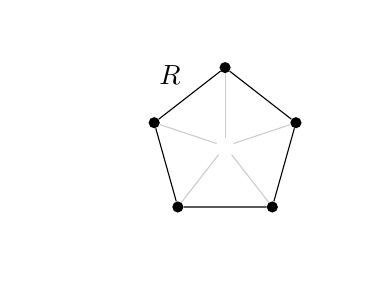
\begin{tikzpicture}
            \draw[fill=white, opacity=0] (-0.5, 0) ellipse (2cm and 1.5cm);
            %\draw[fill=lightgray, draw=black] (0,0) circle (1.25cm);
            %\draw[fill=white] (0,0) circle (0.75cm);
            \node at (-0.7, 0.9) {$R$};
    
            \node[inner sep=1mm] (c) at (0, 0) {$\core$};
            \node[circle, fill, scale=0.015cm] (l1) at (0, 1) { };
            \node[circle, fill, scale=0.015cm] (l2) at (0.9, 0.30) { };
            \node[circle, fill, scale=0.015cm] (l3) at (0.6, -0.77) {};
            \node[circle, fill, scale=0.015cm] (l4) at (-0.6, -0.77) {};
            \node[circle, fill, scale=0.015cm] (l5) at (-0.9, 0.30) {};
    
            \draw[opacity=0.2] (c) -- (l1);
            \draw[opacity=0.2] (c) -- (l2);
            \draw[opacity=0.2] (c) -- (l3);
            \draw[opacity=0.2] (c) -- (l4);
            \draw[opacity=0.2] (c) -- (l5);
            \draw (l1) -- (l2) -- (l3) -- (l4) -- (l5) -- (l1);
        \end{tikzpicture}
    \end{figure}

    Such a coloring might not always be guaranteed.
\end{frame}

\begin{frame}
    \frametitle{Reducers}

    We can add extra vertices on the other side of the ring. This restricts the possible colorings we can encounter.
    \begin{figure}[!h]
        \centering
        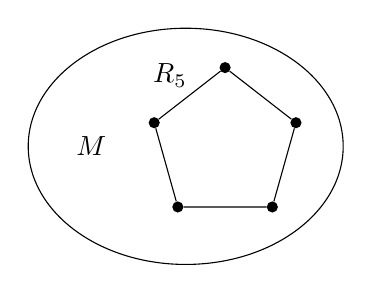
\begin{tikzpicture}
            \draw[fill=white] (-0.5, 0) ellipse (2cm and 1.5cm);
            \node at (-1.7, 0) {$M$};
            \node at (-0.7, 0.9) {$R_5$};
    
            \node[circle, fill, scale=0.015cm] (l1) at (0, 1) { };
            \node[circle, fill, scale=0.015cm] (l2) at (0.9, 0.30) { };
            \node[circle, fill, scale=0.015cm] (l3) at (0.6, -0.77) {};
            \node[circle, fill, scale=0.015cm] (l4) at (-0.6, -0.77) {};
            \node[circle, fill, scale=0.015cm] (l5) at (-0.9, 0.30) {};
    
            \draw (l1) -- (l2) -- (l3) -- (l4) -- (l5) -- (l1);
        \end{tikzpicture}
        \hspace{1cm}
        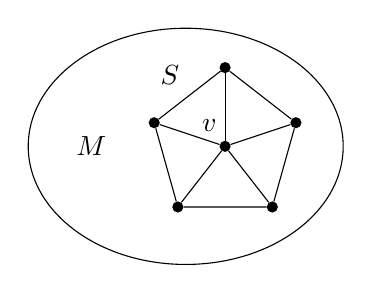
\begin{tikzpicture}
            \draw[fill=white] (-0.5, 0) ellipse (2cm and 1.5cm);
            \node at (-1.7, 0) {$M$};
            \node at (-0.7, 0.9) {$S$};
    
            \node (c) at (-0.2, 0.27) { $v$ };
            \node[circle, fill, scale=0.015cm] (c) at (0, 0) {};
            \node[circle, fill, scale=0.015cm] (l1) at (0, 1) { };
            \node[circle, fill, scale=0.015cm] (l2) at (0.9, 0.30) { };
            \node[circle, fill, scale=0.015cm] (l3) at (0.6, -0.77) {};
            \node[circle, fill, scale=0.015cm] (l4) at (-0.6, -0.77) {};
            \node[circle, fill, scale=0.015cm] (l5) at (-0.9, 0.30) {};
    
            \draw (c) -- (l1);
            \draw (c) -- (l2);
            \draw (c) -- (l3);
            \draw (c) -- (l4);
            \draw (c) -- (l5);
            \draw (l1) -- (l2) -- (l3) -- (l4) -- (l5) -- (l1);
        \end{tikzpicture}
        \caption{A graph that supports all ring colorings (left). A graph that only supports 3-colorings (right).}
    \end{figure}
    The ring + extra vertices and edges is a \textit{reducer} graph.
\end{frame}

\begin{frame}
    \frametitle{Reducers}
    We restrict the size of the reducers such that $|S-R| \leq k$. By increasing $k$, we get more control but a larger graph to color.
    \begin{block}{Reducer Size}
    \begin{itemize}
        \item If $k=0$, then $S=R$ and we reduce to $M+R$ and $\core+R$. This is the smallest possible reduction and ideal situation.
        \item If $k=1$, then we can set $S=R+v$. Our reduced graph is then one vertex larger.
        \item If $k \geq |\confg|$, then there is no point in reducing, since we obtain the same graph $M+\confg$.
    \end{itemize}
\end{block}
\end{frame}

\begin{frame}
    \frametitle{$k$-Reducibility}
    \begin{definition}<1->
        A configuration $\confg=\core+R$ is \emph{$k$-reducible} if for all planar graphs $G=M+\confg$ and some reducers $S$ and $S'$ on $\leq k < |\confg|$ vertices, there exists a common ring coloring for $M+S$ and $\core+S'$.
    \end{definition}
    \begin{definition}<2->
        The ring $R_n$ is \emph{$k$-reducible} if all configurations $\confg$ on $R_n$ are at most $k$-reducible.
    \end{definition}
\end{frame}

\begin{frame}
    \frametitle{$k$-reducibility}
    \begin{example}
        The rings $R_2$ and $R_3$ are 0-reducible. The only colorings are $ab$ and $abc$. Therefore, there is always a common ring coloring for $M+R$ and $\core+R$.
    \end{example}
    \vspace{1cm}
    We will be proving the 0-reducibility of $R_4$ and the 1-reducibility of $R_5$ after introducing Kempe-chains.
\end{frame}